\documentclass[11pt,letterpaper]{article}

% Load some basic packages that are useful to have
% and that should be part of any LaTeX installation.
%
% be able to include figures
\usepackage{graphicx}
% get nice colors
\usepackage{xcolor}

% change default font to Palatino (looks nicer!)
\usepackage{apjfonts}
% load some useful math symbols/fonts
\usepackage{latexsym,amsfonts,amsmath,amssymb}

% comfort package to easily set margins
\usepackage[top=1in, bottom=1in, left=1in, right=1in]{geometry}

% control some spacings
%
% spacing after a paragraph
\setlength{\parskip}{.15cm}
% indentation at the top of a new paragraph
\setlength{\parindent}{0.0cm}


\begin{document}

\begin{center}
\Large
{\bf Ay190 -- Worksheet 8} \\
\large
Xiangcheng Ma \\
Date: \today
\end{center}

\section*{Stellar Structure}
(a) The core of this routine is a loop doing intergration from stellar center to an outer radius by a number of steps. For each step, we use the function ``{\tt tov\_integrate\_FE}" (the name would change for other mathods) to do the integration from $i^{th}$ step to $(i+1)^{th}$ step.

(b) See my implementations in the code.

(c) I implement RK2, RK3 and RK4 method in the original code, please find them therein. In the next question, I will use RK4 run for the plot. Note that to avoid data outflow, I choose a small value $1\times10^{-8}$ instead of $0$ for a start.

(d) I plot the density $\rho(r)$ and accumulated mass $M(r)$ against radius $r$ in Figure~\ref{fig}. I omit the pressure since it is simply related to density.

\begin{figure}[ht]
\centering
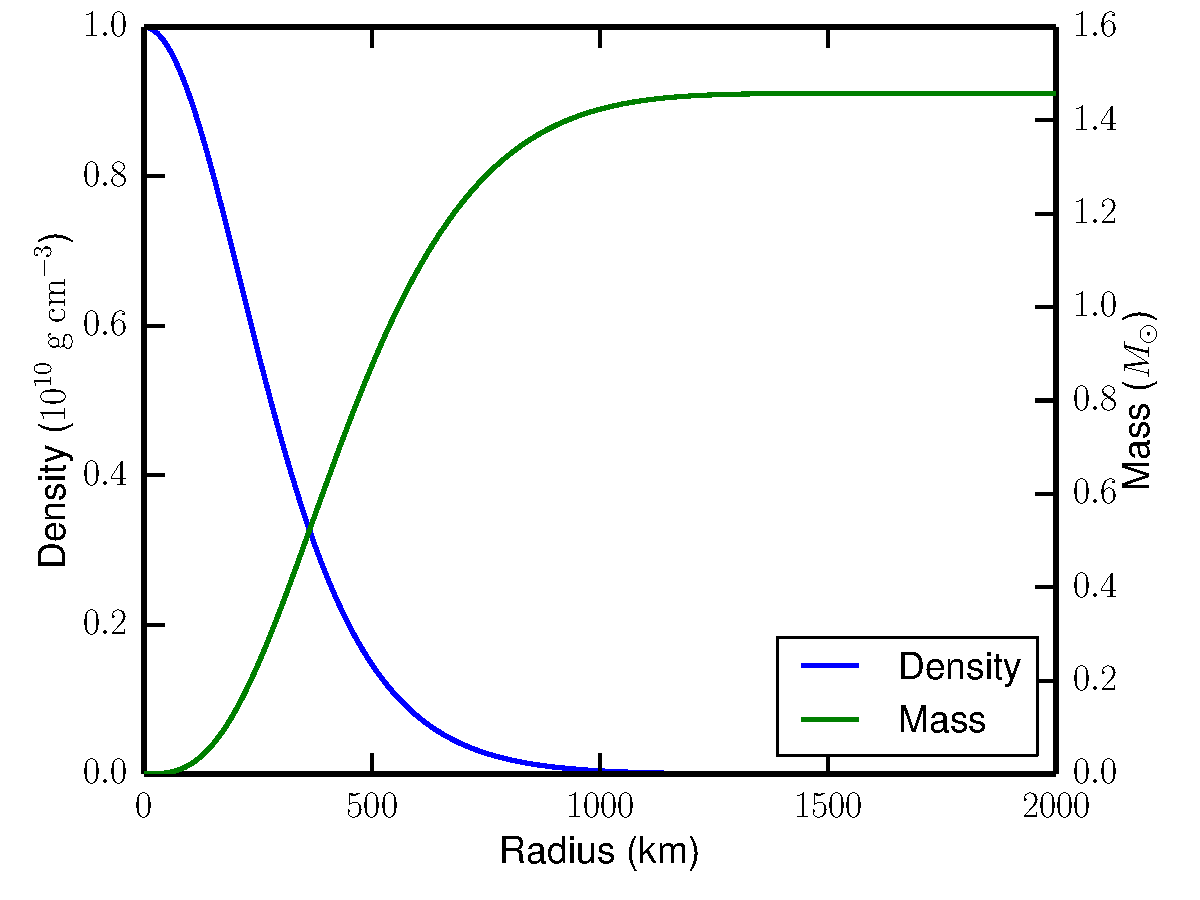
\includegraphics[width=0.9\textwidth]{fig.pdf}
\caption{Stellar Structure}
\label{fig}
\end{figure}

\end{document}
